%%%%%%%%%%%%%%%%%%%%%%%%%%%%%%%%%%%%%%%%%%%%%%%%%%%%%%%%%%%%%%%%%%%%%%%%%%%%%%%%%%
\begin{frame}[fragile]\frametitle{}
\begin{center}
{\Large Data Exploration - Customer Churn}
\end{center}

{\tiny (Ref: mlcourse.ai Demo 1 – Open Machine Learning Course) }
\end{frame}

%%%%%%%%%%%%%%%%%%%%%%%%%%%%%%%%%%%%%%%%%%%%%%%%%%%%%%%%%%
\begin{frame}[fragile]\frametitle{Read Data}	
\begin{lstlisting}
import numpy as np
import pandas as pd
# we don't like warnings
# you can comment the following 2 lines if you'd like to
import warnings
warnings.filterwarnings('ignore')

df = pd.read_csv('data/telecom_churn.csv')
\end{lstlisting}
\end{frame}


%%%%%%%%%%%%%%%%%%%%%%%%%%%%%%%%%%%%%%%%%%%%%%%%%%%%%%%%%%
\begin{frame}[fragile]\frametitle{Read Data}	
Take a look at the first 5 lines using the head method:
\begin{lstlisting}
df.head()
\end{lstlisting}
\begin{center}
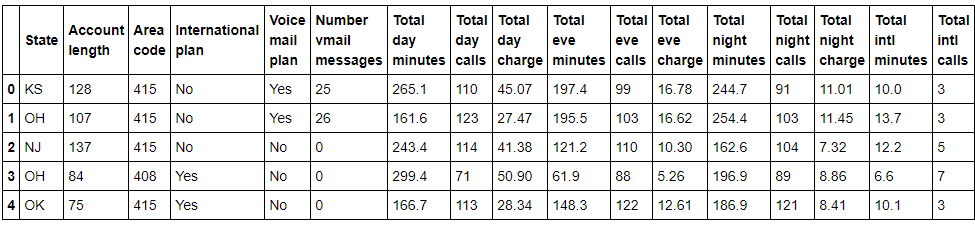
\includegraphics[width=\linewidth,keepaspectratio]{churn1}
\end{center}
Recall that each row corresponds to one client and columns are features of the object.
\end{frame}

%%%%%%%%%%%%%%%%%%%%%%%%%%%%%%%%%%%%%%%%%%%%%%%%%%%%%%%%%%
\begin{frame}[fragile]\frametitle{Let's have a look at data dimensionality}	
\begin{lstlisting}
print(df.shape)

>> (3333, 20)
\end{lstlisting}
From the output, we can see that the table contains 3333 rows and 20 columns. 
\end{frame}

%%%%%%%%%%%%%%%%%%%%%%%%%%%%%%%%%%%%%%%%%%%%%%%%%%%%%%%%%%
\begin{frame}[fragile]\frametitle{Let's have a look at Columns}	
Now let's try printing out the column names using columns:
\begin{lstlisting}
print(df.columns)

>>Index(['State', 'Account length', 'Area code', 'International plan',
       'Voice mail plan', 'Number vmail messages', 'Total day minutes',
       'Total day calls', 'Total day charge', 'Total eve minutes',
       'Total eve calls', 'Total eve charge', 'Total night minutes',
       'Total night calls', 'Total night charge', 'Total intl minutes',
       'Total intl calls', 'Total intl charge', 'Customer service calls',
       'Churn'],
      dtype='object')
\end{lstlisting}
\end{frame}

%%%%%%%%%%%%%%%%%%%%%%%%%%%%%%%%%%%%%%%%%%%%%%%%%%%%%%%%%%
\begin{frame}[fragile]\frametitle{Let's have a look info of Columns}	
We can use the info() method for general information:
\begin{lstlisting}
print(df.info())

>><class 'pandas.core.frame.DataFrame'>
RangeIndex: 3333 entries, 0 to 3332
Data columns (total 20 columns):
State                     3333 non-null object
Account length            3333 non-null int64
Area code                 3333 non-null int64
:
Total intl minutes        3333 non-null float64
Total intl calls          3333 non-null int64
Total intl charge         3333 non-null float64
Customer service calls    3333 non-null int64
Churn                     3333 non-null bool
dtypes: bool(1), float64(8), int64(8), object(3)
\end{lstlisting}
Using this we can find missing values. Here, there are none because each column contains 3333 observations, the same number of rows we saw before with shape.
\end{frame}


%%%%%%%%%%%%%%%%%%%%%%%%%%%%%%%%%%%%%%%%%%%%%%%%%%%%%%%%%%
\begin{frame}[fragile]\frametitle{Describe Data}	
The describe method shows basic statistical characteristics of each numerical feature (int64 and float64 types)
\begin{lstlisting}
df.describe()
\end{lstlisting}
\begin{center}
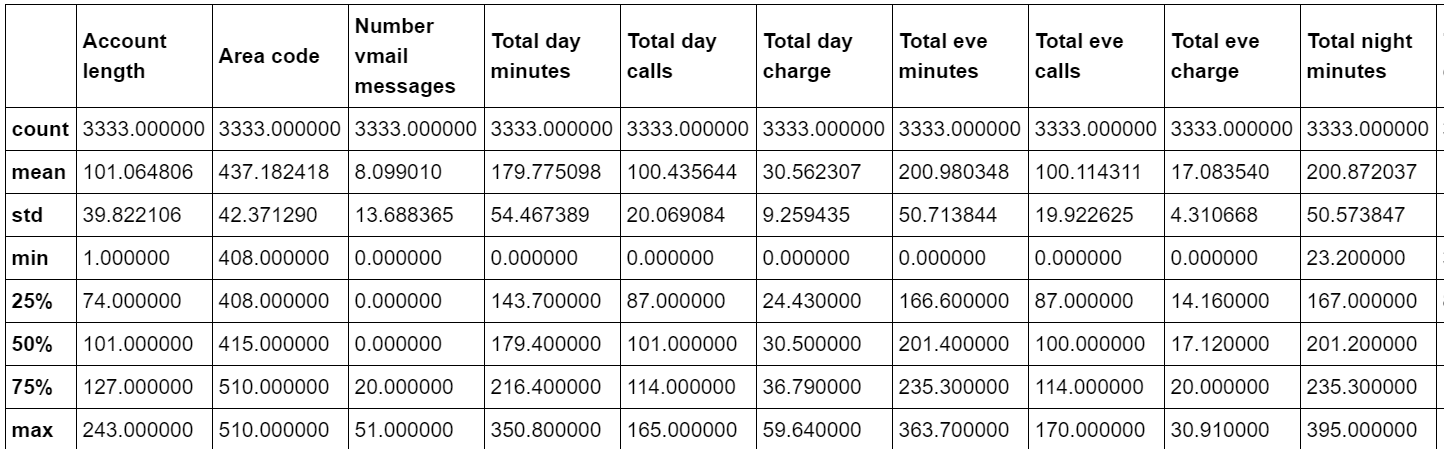
\includegraphics[width=\linewidth,keepaspectratio]{churn2}
\end{center}
\end{frame}

%%%%%%%%%%%%%%%%%%%%%%%%%%%%%%%%%%%%%%%%%%%%%%%%%%%%%%%%%%
\begin{frame}[fragile]\frametitle{Describe Data}	
In order to see statistics on non-numerical features, one has to explicitly indicate data types of interest in the include parameter.
\begin{lstlisting}
df.describe(include=['object', 'bool'])
\end{lstlisting}
\begin{center}
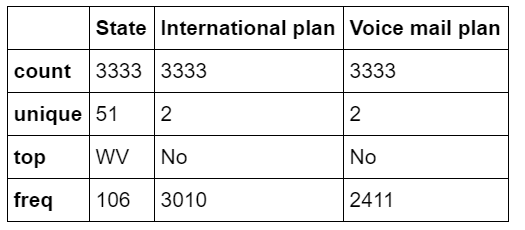
\includegraphics[width=0.5\linewidth,keepaspectratio]{churn3}
\end{center}
\end{frame}

%%%%%%%%%%%%%%%%%%%%%%%%%%%%%%%%%%%%%%%%%%%%%%%%%%%%%%%%%%
\begin{frame}[fragile]\frametitle{Value Counts}	
For categorical (type object) and boolean (type bool) features we can use the value\_counts method. Let’s have a look at the distribution of Churn:
\begin{lstlisting}
df['Churn'].value_counts()

>>
0    2850
1     483
Name: Churn, dtype: int64
\end{lstlisting}
2850 users out of 3333 are loyal; their Churn value is 0.
\end{frame}

%%%%%%%%%%%%%%%%%%%%%%%%%%%%%%%%%%%%%%%%%%%%%%%%%%%%%%%%%%
\begin{frame}[fragile]\frametitle{Value Counts}	
 To calculate the proportion, pass normalize=True to the value\_counts function.
\begin{lstlisting}
df['Churn'].value_counts(normalize=True)

>>
0    0.855086
1    0.144914
Name: Churn, dtype: float64
\end{lstlisting}
2850 users out of 3333 are loyal; their Churn value is 0. To calculate the proportion, pass normalize=True to the value\_counts function.
\end{frame}

%%%%%%%%%%%%%%%%%%%%%%%%%%%%%%%%%%%%%%%%%%%%%%%%%%%%%%%%%%
\begin{frame}[fragile]\frametitle{Sorting}	
A DataFrame can be sorted by the value of one of the variables (i.e columns). For example, we can sort by Total day charge (use ascending=False to sort in descending order):
\begin{lstlisting}
df.sort_values(by='Total day charge', ascending=False).head()
\end{lstlisting}
\begin{center}
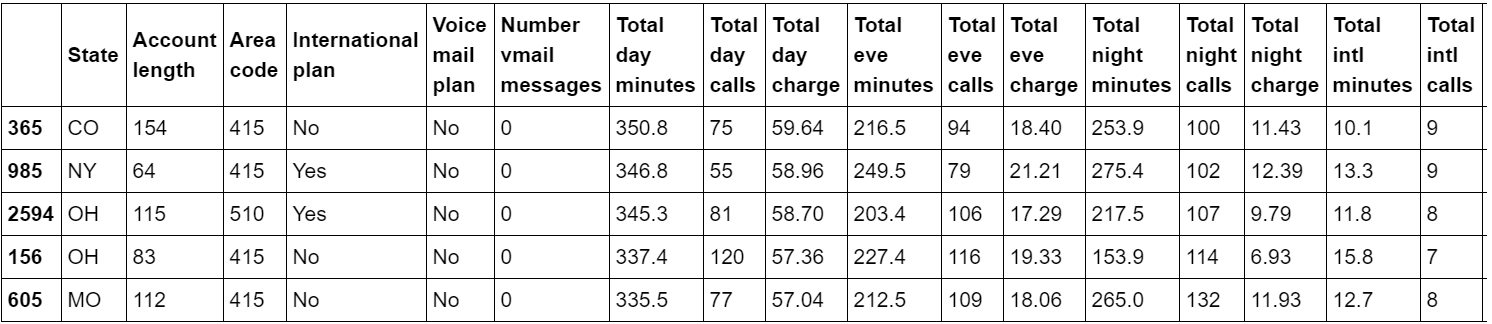
\includegraphics[width=\linewidth,keepaspectratio]{churn4}
\end{center}
\end{frame}

%%%%%%%%%%%%%%%%%%%%%%%%%%%%%%%%%%%%%%%%%%%%%%%%%%%%%%%%%%
\begin{frame}[fragile]\frametitle{Sorting}	
Alternatively, we can also sort by multiple columns:
\begin{lstlisting}
df.sort_values(by=['Churn', 'Total day charge'],
        ascending=[True, False]).head()
\end{lstlisting}
\begin{center}
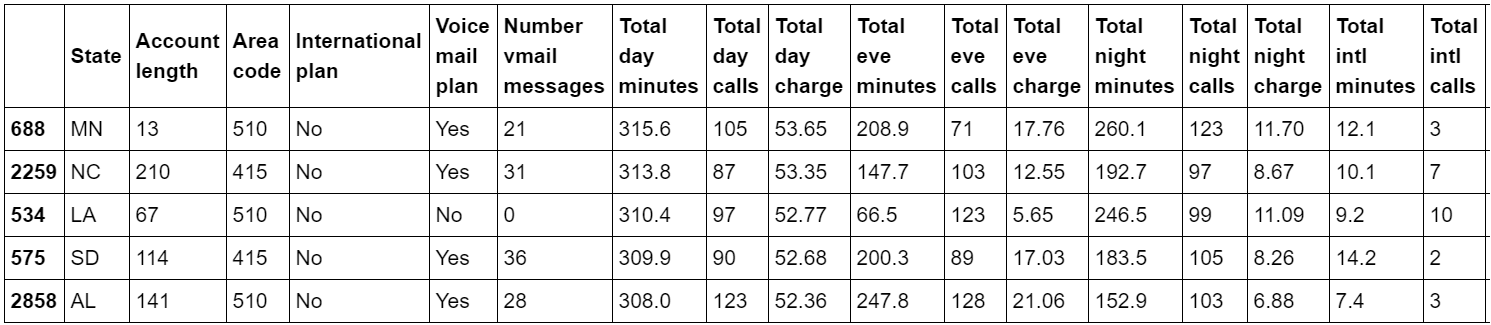
\includegraphics[width=\linewidth,keepaspectratio]{churn5}
\end{center}
\end{frame}

%%%%%%%%%%%%%%%%%%%%%%%%%%%%%%%%%%%%%%%%%%%%%%%%%%%%%%%%%%
\begin{frame}[fragile]\frametitle{Indexing and retrieving data}	
DataFrame can be indexed in different ways.

To get a single column, you can use a DataFrame['Name'] construction. Let's use this to answer a question about that column alone: what is the proportion of churned users in our dataframe?
\begin{lstlisting}
df['Churn'].mean()

>> 0.14491449144914492
\end{lstlisting}

14.5\% is actually quite bad for a company; such a churn rate can make the company go bankrupt.
\end{frame}


%%%%%%%%%%%%%%%%%%%%%%%%%%%%%%%%%%%%%%%%%%%%%%%%%%%%%%%%%%
\begin{frame}[fragile]\frametitle{Boolean indexing}	
\begin{itemize}
\item Boolean indexing with one column is also very convenient. 
\item The syntax is df[P(df['Name'])], where P is some logical condition that is checked for each element of the Name column. 
\item The result of such indexing is the DataFrame consisting only of rows that satisfy the P condition on the Name column.
\end{itemize}

\end{frame}


%%%%%%%%%%%%%%%%%%%%%%%%%%%%%%%%%%%%%%%%%%%%%%%%%%%%%%%%%%
\begin{frame}[fragile]\frametitle{Let's answer}	
What are average values of numerical variables for churned users?

\begin{lstlisting}
df[df['Churn'] == 1].mean()

>> 
Account length            102.664596
Area code                 437.817805
Number vmail messages       5.115942
Total day minutes         206.914079
:
Total intl charge           2.889545
Customer service calls      2.229814
Churn                       1.000000
dtype: float64

\end{lstlisting}
\end{frame}

%%%%%%%%%%%%%%%%%%%%%%%%%%%%%%%%%%%%%%%%%%%%%%%%%%%%%%%%%%
\begin{frame}[fragile]\frametitle{Let's answer}	
How much time (on average) do churned users spend on phone during daytime?

\begin{lstlisting}
df[df['Churn'] == 1]['Total day minutes'].mean()
>> 
206.91407867494814
\end{lstlisting}
\end{frame}

%%%%%%%%%%%%%%%%%%%%%%%%%%%%%%%%%%%%%%%%%%%%%%%%%%%%%%%%%%
\begin{frame}[fragile]\frametitle{Let's answer}	
What is the maximum length of international calls among loyal users (Churn == 0) who do not have an international plan?
\begin{lstlisting}
df[(df['Churn'] == 0) & (df['International plan'] == 'No')]['Total intl minutes'].max()

>> 
18.9
\end{lstlisting}
\end{frame}

%%%%%%%%%%%%%%%%%%%%%%%%%%%%%%%%%%%%%%%%%%%%%%%%%%%%%%%%%%
\begin{frame}[fragile]\frametitle{Indexing}	
\begin{itemize}
\item DataFrames can be indexed by column name (label) or row name (index) or by the serial number of a row. 
\item The loc method is used for indexing by name, while iloc() is used for indexing by number.
\end{itemize}

\end{frame}

%%%%%%%%%%%%%%%%%%%%%%%%%%%%%%%%%%%%%%%%%%%%%%%%%%%%%%%%%%
\begin{frame}[fragile]\frametitle{Let's answer}	
Give us the values of the rows with index from 0 to 5 (inclusive) and columns labeled from State to Area code (inclusive):
\begin{lstlisting}
df.loc[0:5, 'State':'Area code']
\end{lstlisting}
\begin{center}
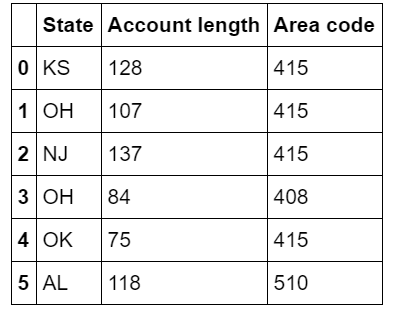
\includegraphics[width=0.5\linewidth,keepaspectratio]{churn6}
\end{center}
\end{frame}

%%%%%%%%%%%%%%%%%%%%%%%%%%%%%%%%%%%%%%%%%%%%%%%%%%%%%%%%%
\begin{frame}[fragile]\frametitle{Let's answer}	
Alternatively
\begin{lstlisting}
df.iloc[0:5, 0:3]
\end{lstlisting}
\begin{center}
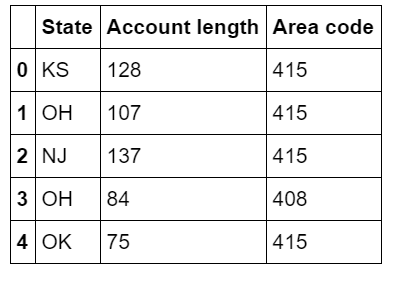
\includegraphics[width=0.5\linewidth,keepaspectratio]{churn7}
\end{center}
\end{frame}

%%%%%%%%%%%%%%%%%%%%%%%%%%%%%%%%%%%%%%%%%%%%%%%%%%%%%%%%%
\begin{frame}[fragile]\frametitle{Let's answer}	
If we need the first or last line of the data frame, we can use the df[:1] or df[-1:] construct:
\begin{lstlisting}
df[-1:]
\end{lstlisting}
\begin{center}
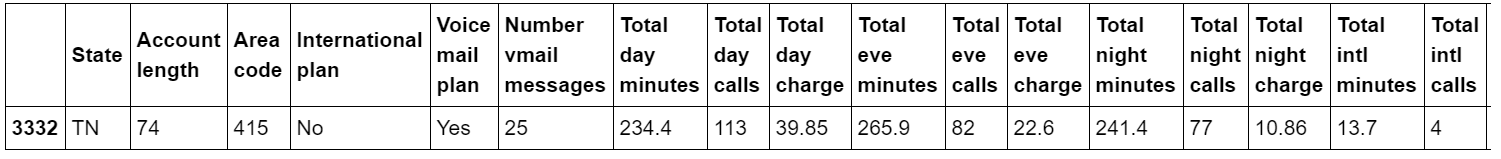
\includegraphics[width=\linewidth,keepaspectratio]{churn8}
\end{center}
\end{frame}

%%%%%%%%%%%%%%%%%%%%%%%%%%%%%%%%%%%%%%%%%%%%%%%%%%%%%%%%%%
\begin{frame}[fragile]\frametitle{Applying Functions to Cells, Columns and Rows}	
To apply functions to each column, use apply():
\begin{lstlisting}
df.apply(np.max)
>> 
State                        WY
Account length              243
Area code                   510
International plan          Yes
:
Total intl calls             20
Total intl charge           5.4
Customer service calls        9
Churn                         1
dtype: object
\end{lstlisting}
\end{frame}

%%%%%%%%%%%%%%%%%%%%%%%%%%%%%%%%%%%%%%%%%%%%%%%%%%%%%%%%%
\begin{frame}[fragile]\frametitle{Applying Functions to Cells, Columns and Rows}	
The apply method can also be used to apply a function to each line. To do this, specify axis=1. Lambda functions are very convenient in such scenarios. For example, if we need to select all states starting with W, we can do it like this:
\begin{lstlisting}
df[df['State'].apply(lambda state: state[0] == 'W')].head()
\end{lstlisting}
\begin{center}
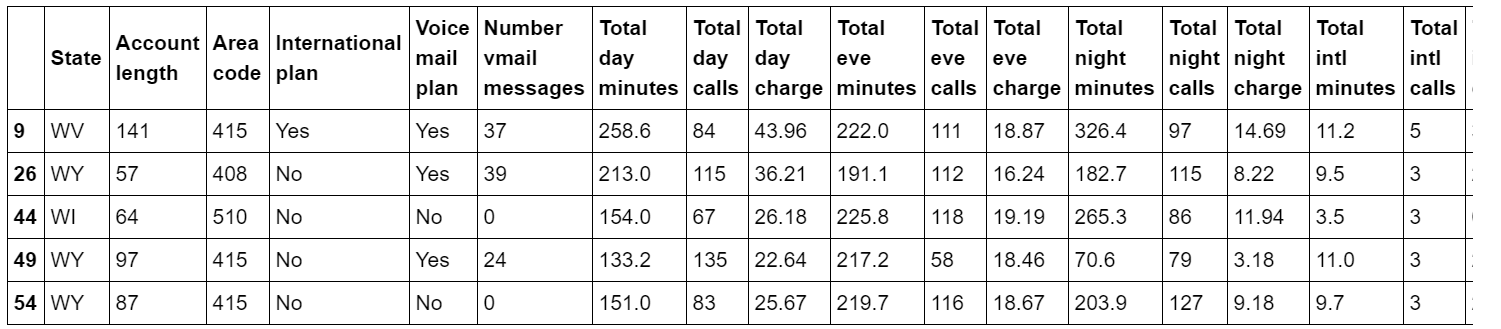
\includegraphics[width=0.8\linewidth,keepaspectratio]{churn9}
\end{center}
\end{frame}

%%%%%%%%%%%%%%%%%%%%%%%%%%%%%%%%%%%%%%%%%%%%%%%%%%%%%%%%%
\begin{frame}[fragile]\frametitle{Map}	
The map method can be used to replace values in a column by passing a dictionary of the form {old\_value: new\_value} as its argument:
\begin{lstlisting}
d = {'No' : False, 'Yes' : True}
df['International plan'] = df['International plan'].map(d)
df.head()
\end{lstlisting}
\begin{center}
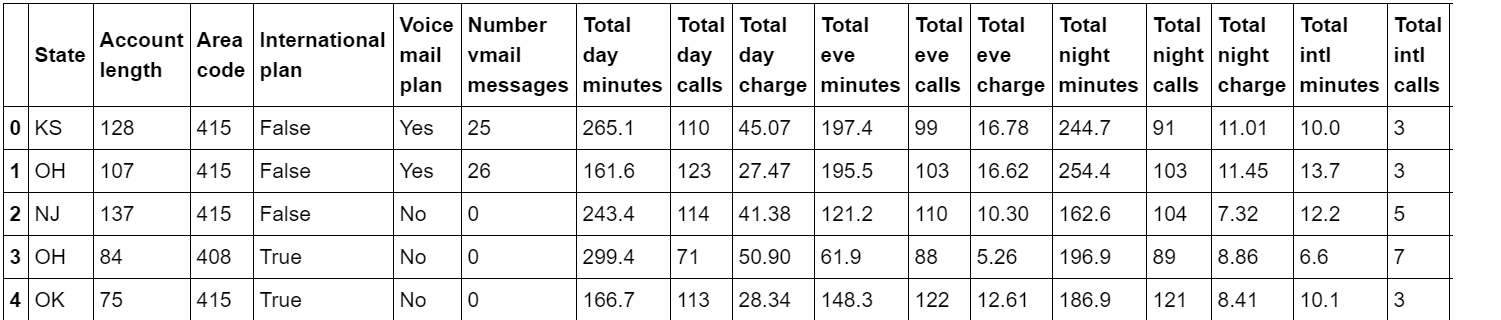
\includegraphics[width=0.8\linewidth,keepaspectratio]{churn10}
\end{center}
\end{frame}

%%%%%%%%%%%%%%%%%%%%%%%%%%%%%%%%%%%%%%%%%%%%%%%%%%%%%%%%%
\begin{frame}[fragile]\frametitle{Replace}	
The same thing can be done with the replace method:
\begin{lstlisting}
df = df.replace({'Voice mail plan': d})
df.head()
\end{lstlisting}
\begin{center}
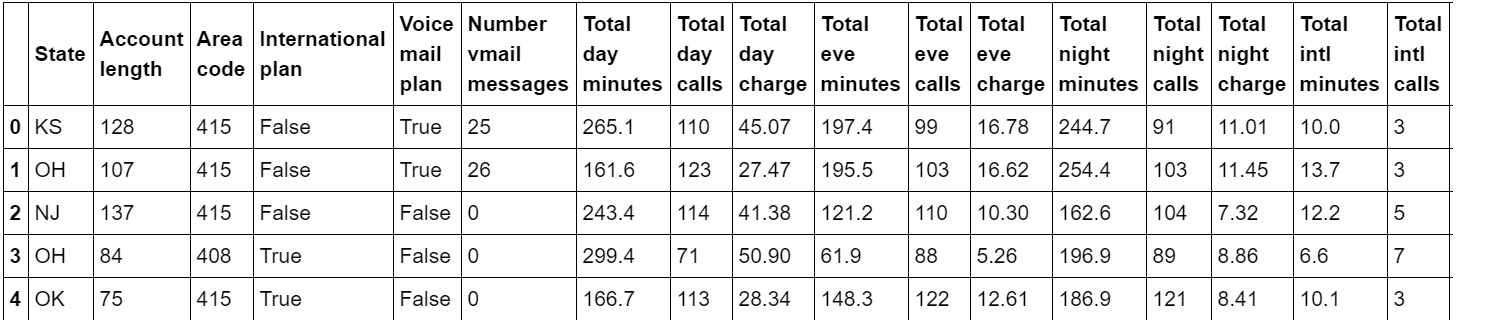
\includegraphics[width=0.8\linewidth,keepaspectratio]{churn11}
\end{center}
\end{frame}

%%%%%%%%%%%%%%%%%%%%%%%%%%%%%%%%%%%%%%%%%%%%%%%%%%%%%%%%%
\begin{frame}[fragile]\frametitle{Grouping}	
In general, grouping data in Pandas goes as follows:
\begin{lstlisting}
df.groupby(by=grouping_columns)[columns_to_show].function()
\end{lstlisting}
\begin{itemize}
\item First, the groupby method divides the grouping\_columns by their values. They become a new index in the resulting dataframe.
\item Then, columns of interest are selected (columns\_to\_show). If columns\_to\_show is not included, all non groupby clauses will be included.
\item Finally, one or several functions are applied to the obtained groups per selected columns.
\end{itemize}
\end{frame}


%%%%%%%%%%%%%%%%%%%%%%%%%%%%%%%%%%%%%%%%%%%%%%%%%%%%%%%%%
\begin{frame}[fragile]\frametitle{Grouping}	
Here is an example where we group the data according to the values of the Churn variable and display statistics of three columns in each group:
\begin{lstlisting}
columns_to_show = ['Total day minutes', 'Total eve minutes', 
                   'Total night minutes']

df.groupby(['Churn'])[columns_to_show].describe(percentiles=[])
\end{lstlisting}
\begin{center}
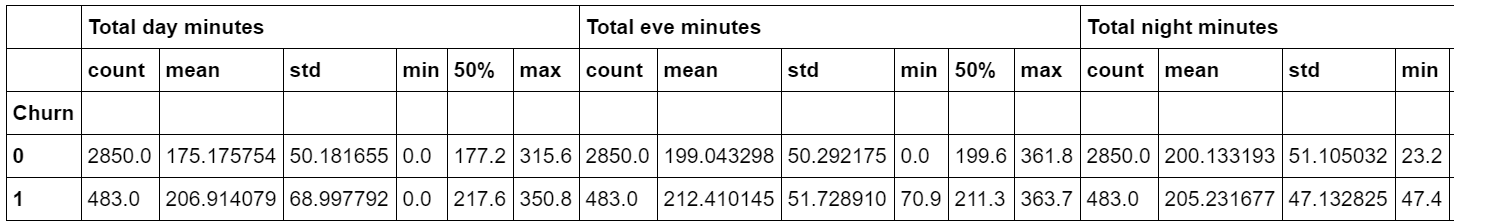
\includegraphics[width=0.8\linewidth,keepaspectratio]{churn12}
\end{center}
\end{frame}


%%%%%%%%%%%%%%%%%%%%%%%%%%%%%%%%%%%%%%%%%%%%%%%%%%%%%%%%%
\begin{frame}[fragile]\frametitle{Grouping}	
Let's do the same thing, but slightly differently by passing a list of functions to agg():
\begin{lstlisting}
columns_to_show = ['Total day minutes', 'Total eve minutes', 
                   'Total night minutes']

df.groupby(['Churn'])[columns_to_show].agg([np.mean, np.std, np.min, np.max])
\end{lstlisting}
\begin{center}
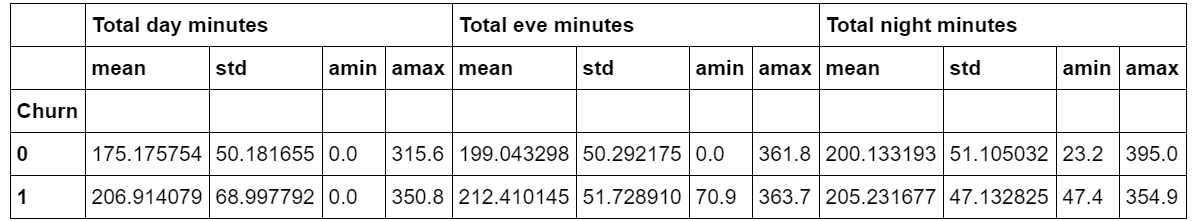
\includegraphics[width=0.8\linewidth,keepaspectratio]{churn13}
\end{center}
\end{frame}

%%%%%%%%%%%%%%%%%%%%%%%%%%%%%%%%%%%%%%%%%%%%%%%%%%%%%%%%%
\begin{frame}[fragile]\frametitle{Summary tables}	
Suppose we want to see how the observations in our sample are distributed in the context of two variables - Churn and International plan. To do so, we can build a contingency table using the crosstab method:
\begin{lstlisting}
pd.crosstab(df['Churn'], df['International plan'])
\end{lstlisting}
\begin{center}
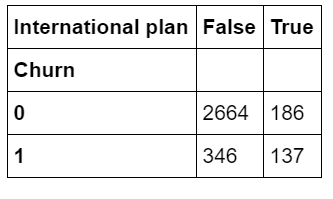
\includegraphics[width=0.35\linewidth,keepaspectratio]{churn14}
\end{center}
\end{frame}

%%%%%%%%%%%%%%%%%%%%%%%%%%%%%%%%%%%%%%%%%%%%%%%%%%%%%%%%%
\begin{frame}[fragile]\frametitle{Summary tables}	
\begin{lstlisting}
pd.crosstab(df['Churn'], df['Voice mail plan'], normalize=True)
\end{lstlisting}
\begin{center}
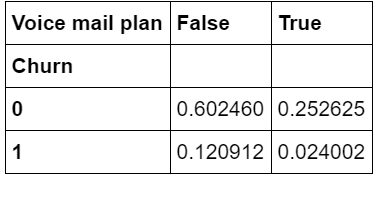
\includegraphics[width=0.35\linewidth,keepaspectratio]{churn15}
\end{center}
We can see that most of the users are loyal and do not use additional services (International Plan/Voice mail).
\end{frame}

%%%%%%%%%%%%%%%%%%%%%%%%%%%%%%%%%%%%%%%%%%%%%%%%%%%%%%%%%
\begin{frame}[fragile]\frametitle{Pivot tables}	
In Pandas, the pivot\_table method takes the following parameters:

\begin{itemize}
\item values - a list of variables to calculate statistics for,
\item index – a list of variables to group data by,
\item aggfunc — what statistics we need to calculate for groups - e.g sum, mean, maximum, minimum or something else.
\end{itemize}
\end{frame}

%%%%%%%%%%%%%%%%%%%%%%%%%%%%%%%%%%%%%%%%%%%%%%%%%%%%%%%%%
\begin{frame}[fragile]\frametitle{Let's answer}	
Let’s take a look at the average number of day, evening, and night calls by area code:
\begin{lstlisting}
df.pivot_table(['Total day calls', 'Total eve calls', 'Total night calls'],
               ['Area code'], aggfunc='mean')
\end{lstlisting}
\begin{center}
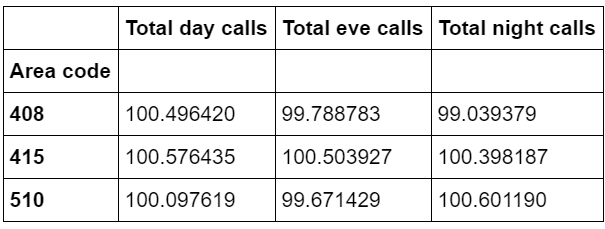
\includegraphics[width=0.5\linewidth,keepaspectratio]{churn16}
\end{center}
\end{frame}

%%%%%%%%%%%%%%%%%%%%%%%%%%%%%%%%%%%%%%%%%%%%%%%%%%%%%%%%%
\begin{frame}[fragile]\frametitle{DataFrame transformations}	
Like many other things in Pandas, adding columns to a DataFrame is doable in many ways.

For example, if we want to calculate the total number of calls for all users, let's create the total\_calls Series and paste it into the DataFrame:
\begin{lstlisting}
total_calls = df['Total day calls'] + df['Total eve calls'] + \
    df['Total night calls'] + df['Total intl calls']
df.insert(loc=len(df.columns), column='Total calls', value=total_calls) 
# loc parameter is the number of columns after which to insert the Series object
# we set it to len(df.columns) to paste it at the very end of the dataframe
df.head()
\end{lstlisting}
\begin{center}
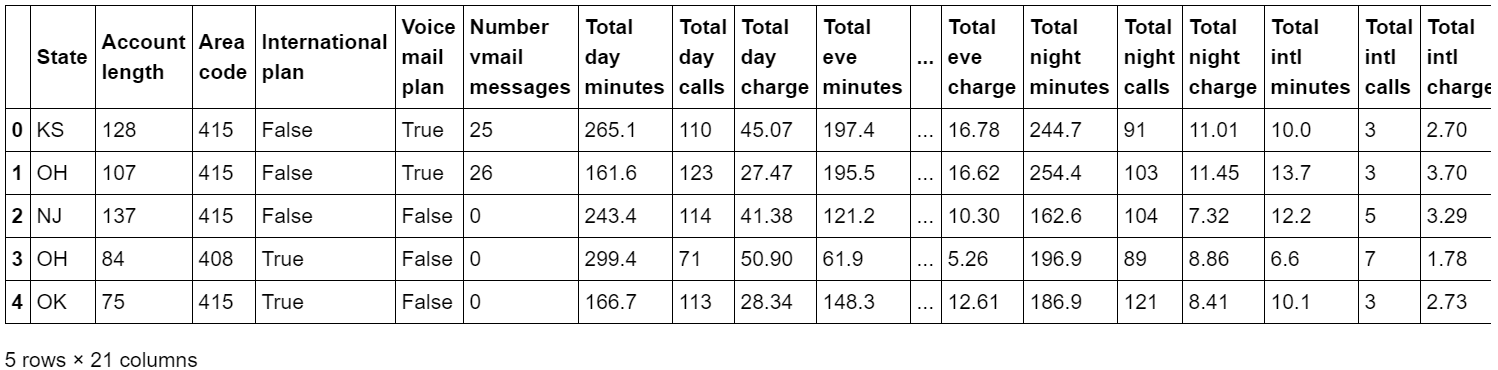
\includegraphics[width=0.7\linewidth,keepaspectratio]{churn17}
\end{center}
\end{frame}

%%%%%%%%%%%%%%%%%%%%%%%%%%%%%%%%%%%%%%%%%%%%%%%%%%%%%%%%%
\begin{frame}[fragile]\frametitle{DataFrame transformations}	
It is possible to add a column more easily without creating an intermediate Series instance:
\begin{lstlisting}
df['Total charge'] = df['Total day charge'] + df['Total eve charge'] + \
    df['Total night charge'] + df['Total intl charge']

df.head()
\end{lstlisting}
\begin{center}
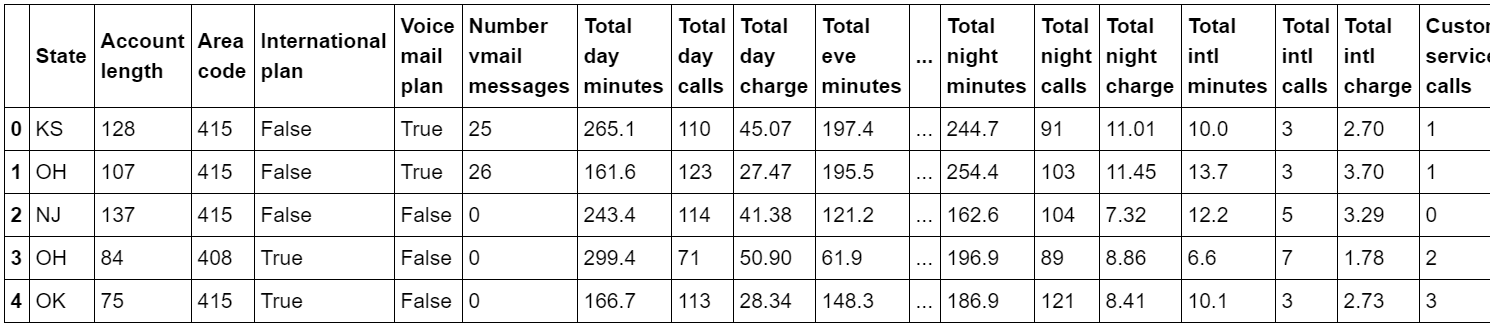
\includegraphics[width=0.7\linewidth,keepaspectratio]{churn18}
\end{center}
\end{frame}

%%%%%%%%%%%%%%%%%%%%%%%%%%%%%%%%%%%%%%%%%%%%%%%%%%%%%%%%%
\begin{frame}[fragile]\frametitle{DataFrame transformations}	
To delete columns or rows, use the drop method, passing the required indexes and the axis parameter (1 if you delete columns, and nothing or 0 if you delete rows). The inplace argument tells whether to change the original DataFrame. With inplace=False, the drop method doesn't change the existing DataFrame and returns a new one with dropped rows or columns. With inplace=True, it alters the DataFrame.
\begin{lstlisting}
# get rid of just created columns
df.drop(['Total charge', 'Total calls'], axis=1, inplace=True) 
# and here's how you can delete rows
df.drop([1, 2]).head() 
\end{lstlisting}
\begin{center}
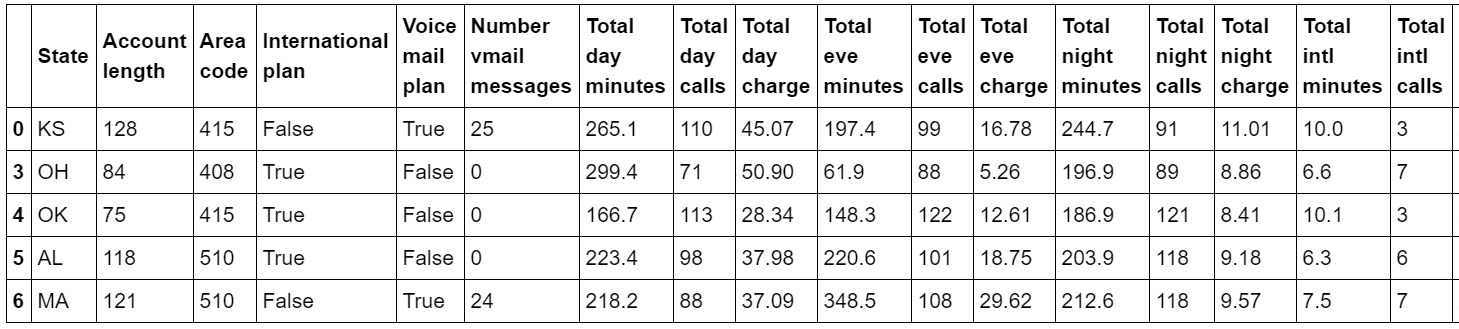
\includegraphics[width=0.7\linewidth,keepaspectratio]{churn19}
\end{center}
\end{frame}

%%%%%%%%%%%%%%%%%%%%%%%%%%%%%%%%%%%%%%%%%%%%%%%%%%%%%%%%%
\begin{frame}[fragile]\frametitle{DataFrame Plotting}	
Let's see how churn rate is related to the International plan variable. We’ll do this using a crosstab contingency table and also through visual analysis with Seaborn (however, visual analysis will be covered more thoroughly in the next article).
\begin{lstlisting}
pd.crosstab(df['Churn'], df['International plan'], margins=True)
\end{lstlisting}
\begin{center}
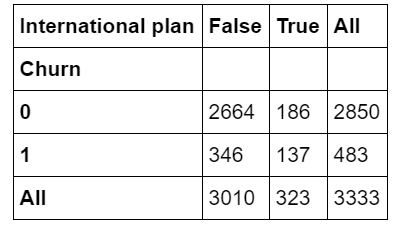
\includegraphics[width=0.5\linewidth,keepaspectratio]{churn20}
\end{center}
\end{frame}


%%%%%%%%%%%%%%%%%%%%%%%%%%%%%%%%%%%%%%%%%%%%%%%%%%%%%%%%%
\begin{frame}[fragile]\frametitle{DataFrame Plotting}	
\begin{lstlisting}
# some imports and "magic" commands to set up plotting 
%matplotlib inline 
import matplotlib.pyplot as plt
# pip install seaborn 
import seaborn as sns
plt.rcParams['image.cmap'] = 'viridis'
sns.countplot(x='International plan', hue='Churn', data=df);
\end{lstlisting}
\begin{center}
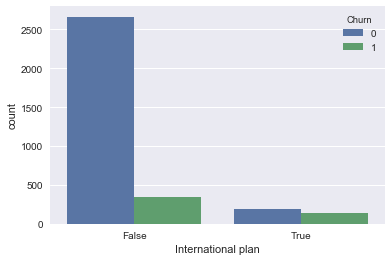
\includegraphics[width=0.5\linewidth,keepaspectratio]{churn21}
\end{center}
We see that, with International Plan, the churn rate is much higher, which is an interesting observation! Perhaps large and poorly controlled expenses with international calls are very conflict-prone and lead to dissatisfaction among the telecom operator's customers.
\end{frame}

%%%%%%%%%%%%%%%%%%%%%%%%%%%%%%%%%%%%%%%%%%%%%%%%%%%%%%%%%
\begin{frame}[fragile]\frametitle{DataFrame Plotting}	
Let’s look at another important feature – Customer service calls. Let’s also make a summary table and a picture.
\begin{lstlisting}
pd.crosstab(df['Churn'], df['Customer service calls'], margins=True)
\end{lstlisting}
\begin{center}
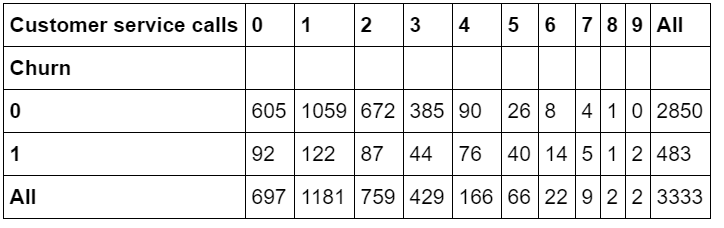
\includegraphics[width=0.7\linewidth,keepaspectratio]{churn22}
\end{center}
\end{frame}

%%%%%%%%%%%%%%%%%%%%%%%%%%%%%%%%%%%%%%%%%%%%%%%%%%%%%%%%%
\begin{frame}[fragile]\frametitle{DataFrame Plotting}	
\begin{lstlisting}
sns.countplot(x='Customer service calls', hue='Churn', data=df);
\end{lstlisting}
\begin{center}
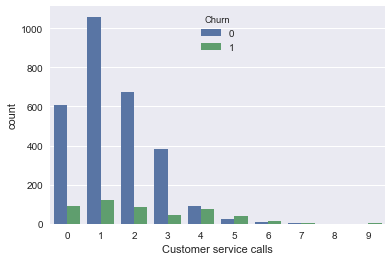
\includegraphics[width=0.7\linewidth,keepaspectratio]{churn23}
\end{center}
Perhaps, it is not so obvious from the summary table, but the picture clearly states that the churn rate strongly increases starting from 4 calls to the service center.
\end{frame}

%%%%%%%%%%%%%%%%%%%%%%%%%%%%%%%%%%%%%%%%%%%%%%%%%%%%%%%%%
\begin{frame}[fragile]\frametitle{Prediction}	
Let’s now add a binary attribute to our DataFrame – Customer service calls > 3. And once again, let's see how it relates to churn.
\begin{lstlisting}
df['Many_service_calls'] = (df['Customer service calls'] > 3).astype('int')

pd.crosstab(df['Many_service_calls'], df['Churn'], margins=True)
\end{lstlisting}
\begin{center}
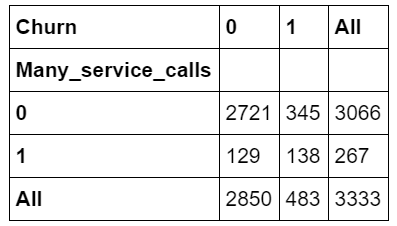
\includegraphics[width=0.5\linewidth,keepaspectratio]{churn24}
\end{center}
\end{frame}

%%%%%%%%%%%%%%%%%%%%%%%%%%%%%%%%%%%%%%%%%%%%%%%%%%%%%%%%%
\begin{frame}[fragile]\frametitle{Prediction}	
\begin{lstlisting}
sns.countplot(x='Many_service_calls', hue='Churn', data=df);
\end{lstlisting}
\begin{center}
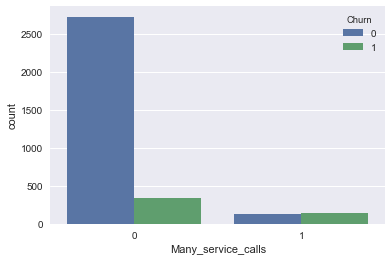
\includegraphics[width=0.5\linewidth,keepaspectratio]{churn25}
\end{center}
\end{frame}

%%%%%%%%%%%%%%%%%%%%%%%%%%%%%%%%%%%%%%%%%%%%%%%%%%%%%%%%%
\begin{frame}[fragile]\frametitle{Prediction}
Let’s construct another contingency table that relates Churn with both International plan and freshly created Many\_service\_calls.	
\begin{lstlisting}
pd.crosstab(df['Many_service_calls'] & df['International plan'] , df['Churn'])
\end{lstlisting}
\begin{center}
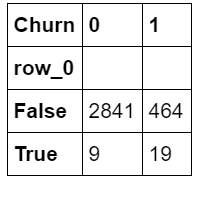
\includegraphics[width=0.3\linewidth,keepaspectratio]{churn26}
\end{center}
\begin{itemize}
\item Therefore, predicting that a customer is loyal (Churn=0) in the case when the number of calls to the service center is less than 4 and the International Plan is added (and predicting Churn=1 otherwise), we might expect an accuracy of 85.8\% (we are mistaken only 464 + 9 times). 
\item This number, 85.8\%, that we got with very simple reasoning serves as a good starting point (baseline) for the further machine learning models that we will build.
\end{itemize}

\end{frame}

%%%%%%%%%%%%%%%%%%%%%%%%%%%%%%%%%%%%%%%%%%%%%%%%%%%%%%%%%
\begin{frame}[fragile]\frametitle{Recap}
\begin{itemize}
\item The share of loyal clients in the sample is 85.5\%. The most naive model that always predicts a ``loyal customer'' on such data will guess right in about 85.5\% of all cases. 
That is, the proportion of correct answers (accuracy) of subsequent models should be no less than this number, and will hopefully be significantly higher;
\item With the help of a simple forecast that can be expressed by the following formula: "International plan = True \& Customer Service calls $> 3 => Churn = 1$, else $Churn = 0$", we can expect a guessing rate of 85.8\%, which is just above 85.5\%. Subsequently, we'll talk about decision trees and figure out how to find such rules automatically based only on the input data;
\end{itemize}

\end{frame}

%%%%%%%%%%%%%%%%%%%%%%%%%%%%%%%%%%%%%%%%%%%%%%%%%%%%%%%%%
\begin{frame}[fragile]\frametitle{Recap}
\begin{itemize}
\item We got these two baselines without applying machine learning, and they’ll serve as the starting point for our subsequent models. If it turns out that with enormous efforts, we increase the share of correct answers by 0.5\% per se, then perhaps we are doing something wrong, and it suffices to confine ourselves to a simple model with two conditions;
\item Before training complex models, it is recommended to manipulate the data a bit, make some plots, and check simple assumptions. Moreover, in business applications of machine learning, they usually start with simple solutions and then experiment with more complex ones.
\end{itemize}

\end{frame}